\documentclass[a4paper,14pt]{extarticle}

\usepackage[utf8x]{inputenc}
\usepackage[T1,T2A]{fontenc}
\usepackage[russian]{babel}
\usepackage{hyperref}
\usepackage{indentfirst}
\usepackage{here}
\usepackage{array}
\usepackage{graphicx}
\usepackage{caption}
\usepackage{subcaption}
\usepackage{chngcntr}
\usepackage{amsmath}
\usepackage{amssymb}
\usepackage{pgfplots}
\usepackage{pgfplotstable}
\usepackage[left=2cm,right=2cm,top=2cm,bottom=2cm,bindingoffset=0cm]{geometry}
\usepackage{multicol}
\usepackage{askmaps}
\usepackage{titlesec}
\usepackage{listings}
\usepackage{color}
\usepackage{courier}

\definecolor{green}{rgb}{0,0.6,0}
\definecolor{gray}{rgb}{0.5,0.5,0.5}
\definecolor{purple}{rgb}{0.58,0,0.82}

\lstset{
	language=Verilog,
	backgroundcolor=\color{white},   
	basicstyle=\small\ttfamily,
	commentstyle=\color{green},
	keywordstyle=\color{blue},	
	numberstyle=\tiny\color{gray},
	stringstyle=\color{purple},
	breakatwhitespace=false,
	breaklines=true,
	captionpos=b,
	keepspaces=true,
	numbers=left,
	numbersep=5pt,
	showspaces=false,
	showstringspaces=false,
	showtabs=false,
	tabsize=4,
	frame=single,
	inputpath={../quartus/},
	literate={~} {$\sim$}{1}
}

\renewcommand{\le}{\ensuremath{\leqslant}}
\renewcommand{\leq}{\ensuremath{\leqslant}}
\renewcommand{\ge}{\ensuremath{\geqslant}}
\renewcommand{\geq}{\ensuremath{\geqslant}}
\renewcommand{\epsilon}{\ensuremath{\varepsilon}}
\renewcommand{\phi}{\ensuremath{\varphi}}
\renewcommand{\thefigure}{\arabic{figure}} 	
\renewcommand*\not[1]{\overline{#1}}

\titleformat*{\section}{\large\bfseries} 
\titleformat*{\subsection}{\normalsize\bfseries} 
\titleformat*{\subsubsection}{\normalsize\bfseries} 
\titleformat*{\paragraph}{\normalsize\bfseries} 
\titleformat*{\subparagraph}{\normalsize\bfseries} 

\counterwithin{figure}{section}
\counterwithin{equation}{section}
\counterwithin{table}{section}
\newcommand{\sign}[1][5cm]{\makebox[#1]{\hrulefill}}
\graphicspath{{../pics/}}
\captionsetup{justification=centering,margin=1cm}
\def\arraystretch{1.3}
\setlength\parindent{5ex}
\titlelabel{\thetitle.\quad}

\begin{document}

\begin{titlepage}
\begin{center}
	Санкт-Петербургский Политехнический Университет Петра Великого\\[0.3cm]
	Институт компьютерных наук и технологий \\[0.3cm]
	Кафедра компьютерных систем и программных технологий\\[4cm]
	
	\textbf{ОТЧЕТ}\\ 
	\textbf{по лабораторной работе}\\[0.5cm]
	\textbf{SystemVerilog №4}\\[0.1cm]
	Автоматизация проектирования\\ дискретных устройств\\[4.0cm]
\end{center}

\begin{flushright}
	\begin{minipage}{0.45\textwidth}
		\textbf{Работу выполнил студент}\\[3mm]
		группа 33501/4 \hspace*{9mm} Дьячков В.В.\\[5mm]
		\textbf{Преподаватель}\\[5mm]
		\sign[1.5cm] \hspace*{1mm} к.т.н., доц. Филиппов А.С. \\[5mm]
	\end{minipage}
\end{flushright}

\vfill

\begin{center}
	Санкт-Петербург\\
	\the\year
\end{center}
\end{titlepage}

\addtocounter{page}{1}
\counterwithin{lstlisting}{section}

\tableofcontents
\newpage
\listoffigures
\lstlistoflistings
\newpage

\section{lab4\_1}

\subsection{Задание}

На языке Verilog опишите устройство, включающее:
\begin{itemize}
	\item Счетчик-делитель, обеспечивающий счет по модулю \code{25 000 000} и формирующий синхронный сигнал переноса (активный уровень сигнала \code{= 1}, длительность один такт тактовой частоты) по достижению счетчиком значения \code{25 000 000 - 1}.
	\item Двоичный, 4-разрядный, счетчик, алгоритм работы, которого задан приведенной ниже таблицей.
\vspace{-0.5cm}
\begin{table}[H]
\begin{center}
	\def\tabcolsep{13pt}
	\caption{Алгоритм работы счетчика}
	\begin{tabular}{|c|c|c|c|c|c|c|}
	\hline	
	\code{aset} & \code{ena} & \code{sclr} & \code{load} & \code{dir} & \code{din} & \code{q} \\ 
	\hline
	\code{0} & \code{X} & \code{X} & \code{X} & \code{X} & \code{X} & Асинхронная установка \\
	\hline
	\code{1} & \code{0} & \code{X} & \code{X} & \code{X} & \code{X} & Хранение \\
	\hline
	\code{1} & \code{1} & \code{0} & \code{X} & \code{X} & \code{X} & Синхронный сброс в \code{0} \\
	\hline
	\code{1} & \code{1} & \code{1} & \code{1} & \code{X} & \code{din} & Запись \code{din} \\
	\hline
	\code{1} & \code{1} & \code{1} & \code{0} & \code{1} & \code{X} & Счет \code{+} \\
	\hline
	\code{1} & \code{1} & \code{1} & \code{0} & \code{0} & \code{X} & Счет \code{-} \\
	\hline
	\end{tabular}
\end{center}
\end{table}	
\vspace{-0.5cm}
	\item Входы:
		\begin{itemize}
			\item Кнопка \code{pba} -- асинхронная установка (установка при нажатии на кнопку). Соединена с входом \code{aset} 4-разрядного счетчика.
			\item Кнопка \code{pbb} -- синхронный сброс (сброс при нажатии на кнопку). Соединена с входом \code{sclr} 4-разрядного счетчика.
			\item Переключатель \code{sw[1]} -- управление загрузкой счетчика. Соединен с входом \code{load} 4-разрядного счетчика.
			\item Переключатель \code{sw[0]} -- управление направлением счета. Соединен с входом \code{dir} 4-разрядного счетчика.
			\item Переключатели \code{sw[7:4]} -- загружаемые данные. Соединены с входом \code{din} 4-разрядного счетчика.
			\item Тактовый сигнал (\code{clk}) подается от тактового генератора (см. описание стенда). Частота тактового сигнала – 25МГц.
		\end{itemize}
	\item Выходы: светодиоды \code{led[7:4]} (двоичного 4-разрядного счетчика).
\end{itemize}

Дополнительные требования:
\begin{itemize}
	\item[$\circ$] Счетчик–делитель и 4-разрядный счетчик описывается в отдельных процедурных блоках.
	\item[$\circ$] При моделировании устройства, с целью сокращения времени моделирования, для счетчика-делителя установите коэффициент деления частоты равным 3 (а не 25 000 000).
\end{itemize}

\subsection{Код на языке Verilog}

В листинге \ref{code:1} приведен код программы на языке Verilog.

\lstinputlisting[caption=lab4\_1.v, label=code:1]{lab4_1/lab4_1.v}

\subsection{Результаты синтеза}

На рис. \ref{fig:lab4_1_rtl} приведено изображение синтезированной схемы в RLT Viewer.

\begin{figure}[H]
\begin{center}
	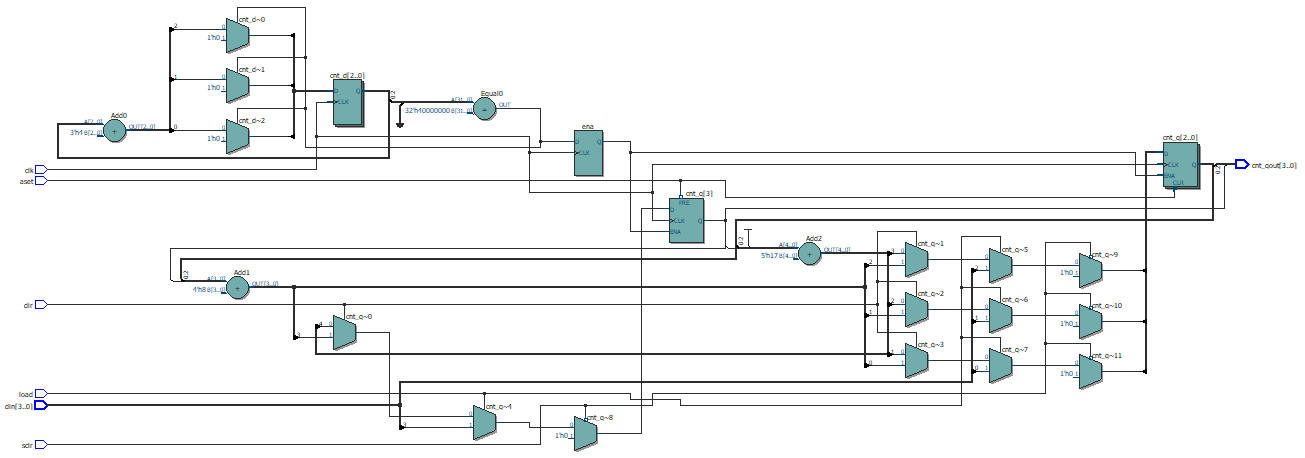
\includegraphics[width=\textwidth]{lab4_1_rtl}
	\caption{Результат синтеза в RLT Viewer}
	\label{fig:lab4_1_rtl}
\end{center}
\end{figure}

\subsection{Результаты моделирования}
\label{sec:lab4_1_modeling}

На рис. \ref{fig:lab4_1_modeling} изображена временная диаграмма работы синтезированного устройства.

\begin{figure}[H]
\begin{center}
	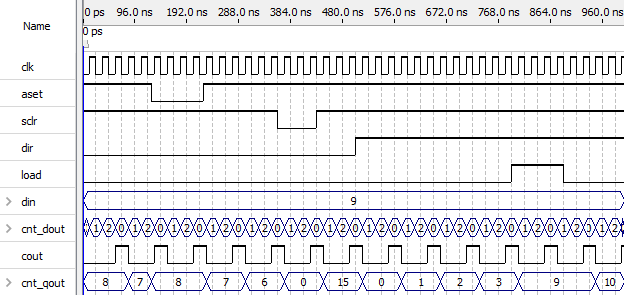
\includegraphics[width=\textwidth]{lab4_1_modeling}
	\caption{Результаты моделирования}
	\label{fig:lab4_1_modeling}
\end{center}
\end{figure}

\newpage

\subsection{Назначение выводов СБИС}

На рис. \ref{fig:lab4_1_pins} приведены назначения выводов СБИС в Pin Planner.

\begin{figure}[H]
\begin{center}
	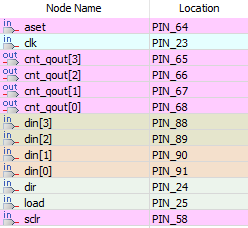
\includegraphics{lab4_1_pins}
	\caption{Таблица назначений в Pin Planer}
	\label{fig:lab4_1_pins}
\end{center}
\end{figure}

\subsection{Результаты проверки на плате}

Для тестирования проекта на плате были использованы тесты, описанные в пункте \ref{sec:lab4_1_modeling}. Результаты тестирования совпадают с ожидаемыми, следовательно, устройство работает верно.

\subsection{Выводы}

Реализовано устройство, содержащее счетчик-делитель и двоичный 4-разрядный счетчик с заданным алгоритмом работы. В описании использовались операторы Concatenate и case. Результаты моделирования и тестирования на плате показали, что разработанное устройство работает верно.

\newpage

\section{lab4\_2}

\subsection{Задание}

На языке Verilog опишите устройство, включающее:
\begin{itemize}
	\item Счетчик-делитель, обеспечивающий счет по модулю \code{25 000 000} и формирующий синхронный сигнал переноса (активный уровень сигнала -- \code{1}, длительность один такт тактовой частоты) по достижению счетчиком значения \code{25 000 000 - 1}.
	\item Регистр сдвига с линейной обратной связью, конфигурация Фибоначчи:
		\begin{itemize}
			\item На вход разрешения работы (\code{ena}) регистра подать сигнал переноса счетчика-делителя.
			\item Полином $x^4 + x^3 + 1$.
		\end{itemize}

	\item Входы:
		\begin{itemize}
			\item Кнопка \code{pba} - асинхронная установка регистра (установка при нажатии на кнопку): один (любой) разряд регистра \code{= 1}, остальные разряды \code{= 0}. 	
			\item Тактовый сигнал (\code{clk}) подается от тактового генератора (см. описание стенда). Частота тактового сигнала – 25МГц.
		\end{itemize}		
	\item Выходы: светодиоды \code{led[3:0]} -- выходы регистра сдвига.
\end{itemize}

Дополнительные требования:
\begin{itemize}
	\item[$\circ$] Счетчик и регистр описываются в отдельных процедурных блоках.
	\item[$\circ$] При моделировании устройства, с целью сокращения времени моделирования, для счетчика-делителя установите коэффициент деления частоты равным \code{3} (а не \code{25 000 000}).
	\item[$\circ$] На результатах моделирования должны отображаться, кроме всех входных сигналов: значение счетчика-делителя, сигнал переноса, значение регистра сдвига.
	\item[$\circ$] По временной диаграмме определите период регистра сдвига
\end{itemize}

В описании можно использовать любые операторы.

\newpage

\subsection{Код на языке Verilog}

В листинге \ref{code:2} приведен код программы на языке Verilog.

\lstinputlisting[caption=lab4\_2.v, label=code:2]{lab4_2/lab4_2.v}
\vspace{-0.5cm}

\subsection{Результаты синтеза}

На рис. \ref{fig:lab4_2_rtl} приведено изображение синтезированной схемы в RLT Viewer.

\begin{figure}[H]
\begin{center}
	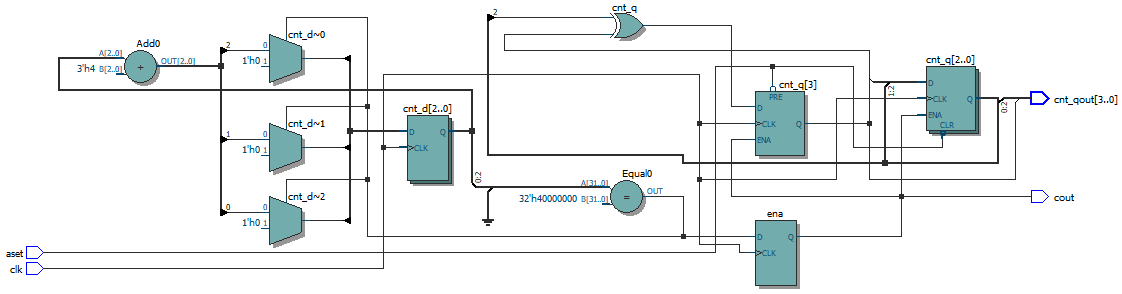
\includegraphics[width=\textwidth]{lab4_2_rtl}
	\caption{Результат синтеза в RLT Viewer}
	\label{fig:lab4_2_rtl}
\end{center}
\end{figure}

\subsection{Результаты моделирования}
\label{sec:lab4_2_modeling}

На рис. \ref{fig:lab4_2_modeling} изображена временная диаграмма работы синтезированного устройства.

\begin{figure}[H]
\begin{center}
	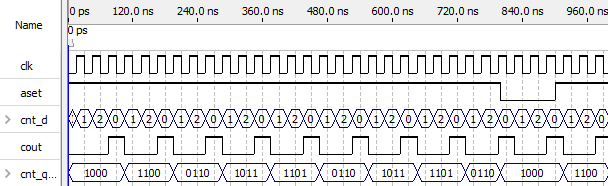
\includegraphics[width=\textwidth]{lab4_2_modeling}
	\caption{Результаты моделирования}
	\label{fig:lab4_2_modeling}
\end{center}
\end{figure}

\subsection{Назначение выводов СБИС}

На рис. \ref{fig:lab4_2_pins} приведены назначения выводов СБИС в Pin Planner.

\begin{figure}[H]
\begin{center}
	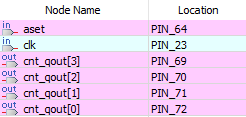
\includegraphics{lab4_2_pins}
	\caption{Таблица назначений в Pin Planer}
	\label{fig:lab4_2_pins}
\end{center}
\end{figure}

\subsection{Результаты проверки на плате}

Для тестирования проекта на плате были использованы тесты, описанные в пункте \ref{sec:lab4_2_modeling}. Результаты тестирования совпадают с ожидаемыми, следовательно, устройство работает верно.

\subsection{Выводы}

Реализовано устройство, содержащее счетчик-делитель и регистр сдвига с линейной обратной связью. Результаты моделирования и тестирования на плате показали, что разработанное устройство работает верно.

\newpage

\section{elab4\_1}

\subsection{Задание}

На языке Verilog опишите устройство, включающее:
\begin{itemize}
	\item Счетчик-делитель, обеспечивающий счет по модулю \code{25 000 000} и формирующий синхронный сигнал переноса (активный уровень сигнала \code{= 1}, длительность один такт тактовой частоты) по достижению счетчиком значения \code{25 000 000 - 1}.
	\item 8-разрядный реверсивный счетчик с динамически изменяемым модулем счета. Вход модуля счета счетчика \code{mod[7:0]} -- соединен с входами \code{sw[7:0]} устройства. Сигналы управления счетчиком заданы приведенной ниже таблицей.
\vspace{-0.5cm}
\begin{table}[H]
\begin{center}
	\def\tabcolsep{13pt}
	\caption{Алгоритм работы счетчика}
	\begin{tabular}{|c|c|c|c|c|}
	\hline	
	\code{ena} & \code{load} & \code{dir} & \code{q} \\ 
	\hline
	\code{0} & \code{X} & \code{X} & Хранение \\
	\hline
	\code{1} & \code{1} & \code{X} & Синхронная загрузка \\
	\hline
	\code{1} & \code{0} & \code{1} & Счет \code{+} \\
	\hline
	\code{1} & \code{0} & \code{0} & Счет \code{-} \\
	\hline
	\end{tabular}
\end{center}
\end{table}	
\vspace{-0.5cm}
	\item Модуль формирования сигнала \code{load} для 8-разрядного реверсивного счетчика -- сигнал \code{load = 1} длительностью \code{1} период тактового сигнала \code{clk} формируется при изменении значения модуля счета, заданного на входах \code{sw[7:0]} устройства.

	\item Входы:
		\begin{itemize}
			\item Переключатели \code{sw[7:0]} -- модуль счета счетчика.
			\item Кнопка \code{pbb} -- кнопка выбора направления счета (если \code{pbb} нажата, то счет на вычитание).
			\item Тактовый сигнал (\code{clk}) подается от тактового генератора (см. описание стенда). Частота тактового сигнала – 25МГц.
		\end{itemize}
	\item Выходы: светодиоды \code{led[7:0]} (выходы двоичного 8-разрядного счетчика).
\end{itemize}

Дополнительные требования:
\begin{itemize}
	\item[$\circ$] Счетчик-делитель, 8-разрядный реверсивный счетчик и модуль формирования сигнала \code{load} описываются в отдельных процедурных блоках.
	\item[$\circ$] При моделировании устройства, с целью сокращения времени моделирования, для счетчика-делителя установите коэффициент деления частоты равным \code{3} (а не \code{25 000 000}).
	\item[$\circ$] На результатах моделирования должны отображаться, кроме всех входных сигналов: значение счетчика-делителя, сигнал переноса, значение 8-разрядного реверсивного счетчика, сигнал \code{load}.
\end{itemize}

В описании можно использовать любые операторы.

\subsection{Код на языке Verilog}

В листинге \ref{code:5} приведен код программы на языке Verilog.

\lstinputlisting[caption=elab4\_1.v, label=code:5]{elab4_1/elab4_1.v}

\subsection{Результаты синтеза}

На рис. \ref{fig:elab4_1_rtl} приведено изображение синтезированной схемы в RLT Viewer.

\begin{figure}[H]
\begin{center}
	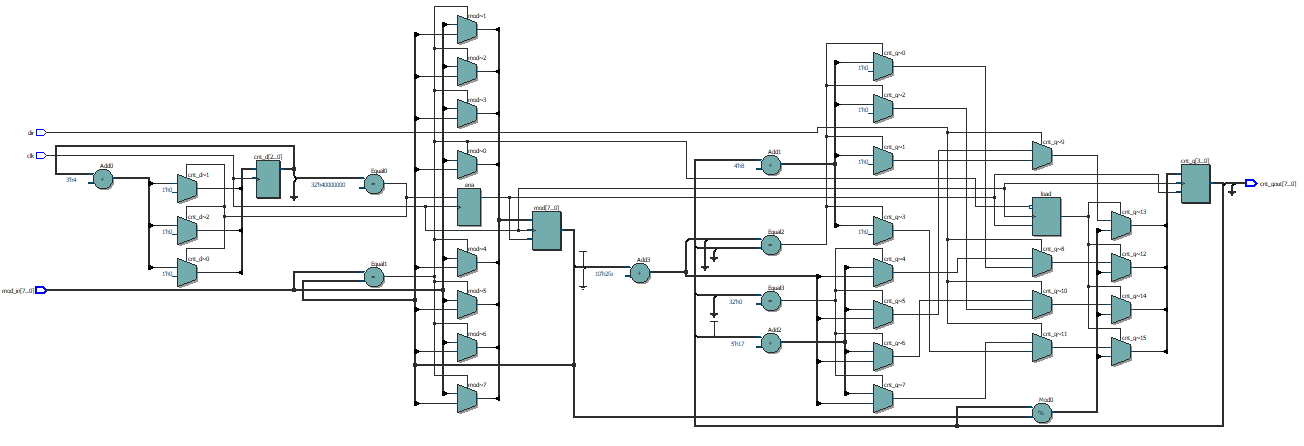
\includegraphics[width=\textwidth]{elab4_1_rtl}
	\caption{Результат синтеза в RLT Viewer}
	\label{fig:elab4_1_rtl}
\end{center}
\end{figure}

\subsection{Результаты моделирования}
\label{sec:elab4_1_modeling}

На рис. \ref{fig:elab4_1_modeling} изображена временная диаграмма работы синтезированного устройства. 

\begin{figure}[H]
\begin{center}
	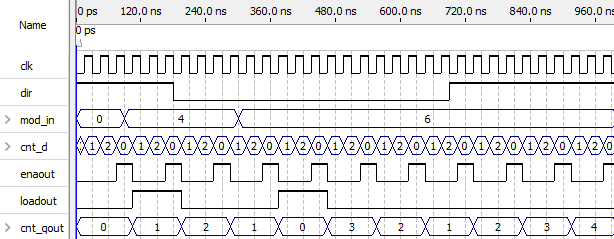
\includegraphics[width=\textwidth]{elab4_1_modeling}
	\caption{Результаты моделирования}
	\label{fig:elab4_1_modeling}
\end{center}
\end{figure}

\subsection{Назначение выводов СБИС}

На рис. \ref{fig:elab4_1_pins} приведены назначения выводов СБИС в Pin Planner.

\begin{figure}[H]
\begin{center}
	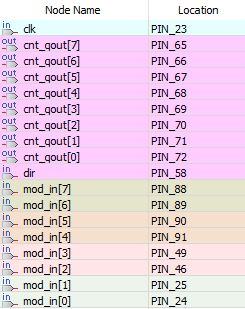
\includegraphics{elab4_1_pins}
	\caption{Таблица назначений в Pin Planer}
	\label{fig:elab4_1_pins}
\end{center}
\end{figure}

\subsection{Результаты проверки на плате}

Для тестирования проекта на плате были использованы тесты, описанные в пункте \ref{sec:elab4_1_modeling}. Результаты тестирования совпадают с ожидаемыми, следовательно, устройство работает верно.

\subsection{Выводы}

Реализовано устройство, содержащее счетчик-делитель и 8-разрядный реверсивный счетчик с динамически изменяемым модулем счета. Результаты моделирования и тестирования на плате показали, что разработанное устройство работает верно.

\end{document}